% Basado en el template realizado por Diego Essaya, disponible en
%                                                         http://lug.fi.uba.ar
% Modificado por Sebastián Santisi.
% 2007: Modificado por Patricio Moreno y Michel Peterson.
% 2014: Modificado por Patricio Moreno.
% 2017: Modificado por Patricio Moreno.
% 2021: Modificado por Carla Sobico.
% 2024: Modificado(simplificado) por Francisco Del Rio.

% Acá se define el tamaño de letra principal:
% Para utilizar los estilos de KOMA-script, desconectar la línea siguiente y
% comentar la que le sigue (dejar sin comentar un único documentclass)
%\documentclass[10pt, spanish]{scrartcl}
\documentclass[a4paper, twoside, 10pt, spanish]{article}

%%%%%%%%%%%%%%%%%%%%%%%%%%%%%%
% CS
%%%%%%%%%%%%%%%%%%%%%%%%%%%%%%
\usepackage{listings}

\usepackage{booktabs}
\usepackage[margin=1in]{geometry}
\usepackage{array}
\usepackage{pdflscape}
\usepackage{multirow}

% CONFIGURACIONES GENERALES
%%%%%%%%%%%%%%%%%%%%%%%%%%%%%%%%%%%%%%%%%%%%%%%%%%%%%%%%%%%%%%%%%%%%%%%%%%%%%
% Definición del tamaño de página y los márgenes:
% Si preferís menos márgenes, descomentá la línea siguiente
%\usepackage[a4paper,headheight=16pt,scale={0.7,0.8},hoffset=0.5cm]{geometry}
\usepackage[demo]{graphicx}
\usepackage{caption}
\usepackage{subcaption}
\usepackage{babel}  % contiene la correcta separación en sílabas del español
\usepackage[utf8x]{inputenc}    % porque el encoding del documento es UTF-8
\usepackage[per-mode=fraction]{siunitx}
\sisetup%
{
	output-decimal-marker = {,},
	exponent-product = \cdot,
    group-digits = integer,
	group-separator = {.}
}


%
% El paquete amsmath agrega algunas funcionalidades extra a las fórmulas.
% Además defino la numeración de las tablas y figuras al estilo "Figura 2.3",
% en lugar de "Figura 7". (Por lo tanto, aunque no uses fórmulas, si querés
% este tipo de numeración dejá el paquete amsmath descomentado).
%
\usepackage{amsmath, amsfonts, amssymb}
%\numberwithin{equation}{section}
%\numberwithin{figure}{section}
\numberwithin{table}{section}
%%%%%%%%%%%%%%%%%%%%%%%%%%%%%%%%%%%%%%%%%%%%%%%%%%%%%%%%%%%%%%%%%%%%%%%%%%%%%

%%%%%%%%%%%%%%%%%%%%%%%%%%%%%%%%%%%%%%%%%%%%%%%%%%%%%%%%%%%%%%%%%%%%%%%%%%%%%
% ENCABEZADO y PIE DE PÁGINA
%%%%%%%%%%%%%%%%%%%%%%%%%%%%%%%%%%%%%%%%%%%%%%%%%%%%%%%%%%%%%%%%%%%%%%%%%%%%%
\usepackage{fancyhdr}   % Para poder personalizarlo
\usepackage{lastpage}   % Para poder saber cuántas páginas tiene el documento
\pagestyle{fancy}
\renewcommand{\sectionmark}[1]{\markboth{}{\thesection\ \ #1}}
\fancyhead{}	% Elimino el contenido del encabezado
% Muestra la sección a la derecha (izquierda) en páginas impares (pares)
\fancyhead[RO,LE]{\rightmark}
% El siguiente texto a la derecha (izquierda) en páginas pares (impares)
\fancyhead[RE,LO]{TA138 - Segundo checkpoint}
\fancyfoot{}	% Elimino el contenido del pie de página
% A la izquierda (derecha) en páginas pares (impares): nro. de página / total
\fancyfoot[LE,RO]{\thepage/\pageref{LastPage}}
%%%%%%%%%%%%%%%%%%%%%%%%%%%%%%%%%%%%%%%%%%%%%%%%%%%%%%%%%%%%%%%%%%%%%%%%%%%%%

%%%%%%%%%%%%%%%%%%%%%%%%%%%%%%%%%%%%%%%%%%%%%%%%%%%%%%%%%%%%%%%%%%%%%%%%%%%%%
% Hipervínculos (enlaces) en el documento (y modificación de atributos)
%%%%%%%%%%%%%%%%%%%%%%%%%%%%%%%%%%%%%%%%%%%%%%%%%%%%%%%%%%%%%%%%%%%%%%%%%%%%%
\usepackage{url}
\urlstyle{tt}
\usepackage[colorlinks=true,linkcolor=black, urlcolor=blue]{hyperref}
\hypersetup{
    breaklinks,
    baseurl       = http://,
    pdfborder     = 0 0 0,
    pdfpagemode   = UseNone,
    pdfstartpage  = 1,
    pdfcreator    = {Plantilla de informe de TP para \LaTeX{}},
    bookmarksopen = true,
    bookmarksdepth= 2,% to show sections and subsections
    pdfauthor     = {Apellido~1, Apellido~2, Apellido~3},
    pdftitle      = {-},
    pdfsubject    = {Informe},
    pdfkeywords   = {}%
    }
%%%%%%%%%%%%%%%%%%%%%%%%%%%%%%%%%%%%%%%%%%%%%%%%%%%%%%%%%%%%%%%%%%%%%%%%%%%%%

%%%%%%%%%%%%%%%%%%%%%%%%%%%%%%%%%%%%%%%%%%%%%%%%%%%%%%%%%%%%%%%%%%%%%%%%%%%%%
% LISTAS (para poder modificar los 'bullets' de las listas)
%%%%%%%%%%%%%%%%%%%%%%%%%%%%%%%%%%%%%%%%%%%%%%%%%%%%%%%%%%%%%%%%%%%%%%%%%%%%%
\usepackage{enumerate}
%%%%%%%%%%%%%%%%%%%%%%%%%%%%%%%%%%%%%%%%%%%%%%%%%%%%%%%%%%%%%%%%%%%%%%%%%%%%%

%%%%%%%%%%%%%%%%%%%%%%%%%%%%%%%%%%%%%%%%%%%%%%%%%%%%%%%%%%%%%%%%%%%%%%%%%%%%%
% TABLAS (para que se vean bien)
%%%%%%%%%%%%%%%%%%%%%%%%%%%%%%%%%%%%%%%%%%%%%%%%%%%%%%%%%%%%%%%%%%%%%%%%%%%%%
\usepackage{booktabs}
\usepackage{multirow}
%%%%%%%%%%%%%%%%%%%%%%%%%%%%%%%%%%%%%%%%%%%%%%%%%%%%%%%%%%%%%%%%%%%%%%%%%%%%%

%%%%%%%%%%%%%%%%%%%%%%%%%%%%%%%%%%%%%%%%%%%%%%%%%%%%%%%%%%%%%%%%%%%%%%%%%%%%%
% IMÁGENES
%%%%%%%%%%%%%%%%%%%%%%%%%%%%%%%%%%%%%%%%%%%%%%%%%%%%%%%%%%%%%%%%%%%%%%%%%%%%%
% Para incluir imágenes, el siguiente código carga el paquete graphicx
% según se esté generando un archivo dvi o un pdf (con pdflatex).

% Para generar dvi, descomentá la linea siguiente:
%\usepackage[dvips]{graphicx}

% Para generar pdf, descomentá las dos lineas seguientes:
\usepackage{graphicx}
\pdfcompresslevel=9

% Todas las imágenes están en el directorio imgs:
\newcommand{\imgdir}{imgs}
\graphicspath{{\imgdir/}}
%%%%%%%%%%%%%%%%%%%%%%%%%%%%%%%%%%%%%%%%%%%%%%%%%%%%%%%%%%%%%%%%%%%%%%%%%%%%%

%%%%%%%%%%%%%%%%%%%%%%%%%%%%%%%%%%%%%%%%%%%%%%%%%%%%%%%%%%%%%%%%%%%%%%%%%%%%%
% DIAGRAMAS DE FLUJO EN DIA
%%%%%%%%%%%%%%%%%%%%%%%%%%%%%%%%%%%%%%%%%%%%%%%%%%%%%%%%%%%%%%%%%%%%%%%%%%%%%
% Necesitas este paquete si haces los diagramas de flujo en el programa Dia
% y exportás a latex
%\usepackage{tikz}
%%%%%%%%%%%%%%%%%%%%%%%%%%%%%%%%%%%%%%%%%%%%%%%%%%%%%%%%%%%%%%%%%%%%%%%%%%%%%

%%%%%%%%%%%%%%%%%%%%%%%%%%%%%%%%%%%%%%%%%%%%%%%%%%%%%%%%%%%%%%%%%%%%%%%%%%%%%
% INSERCIÓN DE CÓDIGO FUENTE
%%%%%%%%%%%%%%%%%%%%%%%%%%%%%%%%%%%%%%%%%%%%%%%%%%%%%%%%%%%%%%%%%%%%%%%%%%%%%
% El paquete recomendado actualmente es minted.
% Documentación: https://www.ctan.org/pkg/minted
\usepackage[
        section,    % Numera el código según la sección
    ]{minted}
% minted provee los comandos:
% 1)  \mint[<opciones>]{<lenguaje>}<delimitador><código><delimitador>
% 2)  \mintinline[<opciones>]{<lenguaje>}<delimitador><código><delimitador>
% 3)  \inputminted[<opciones>]{<lenguaje>}{<archivo>}
\setminted[c]{
%        style=,
        linenos,            % Mostrar los números de línea
        numberfirstline,    % Numerar SIEMPRE la primera línea mostrada
        tabsize=4,          % Reemplazar las tabulaciones por 4 espacios
        autogobble          % Eliminar espacio sobrante al comienzo
    }
%%%%%%%%%%%%%%%%%%%%%%%%%%%%%%%%%%%%%%%%%%%%%%%%%%%%%%%%%%%%%%%%%%%%%%%%%%%%%
% COMANDOS UTILES
%%%%%%%%%%%%%%%%%%%%%%%%%%%%%%%%%%%%%%%%%%%%%%%%%%%%%%%%%%%%%%%%%%%%%%%%%%%%%
% los siguientes comandos permiten escribir de manera uniforme en todo el
% documento

% Para poder manejar los espacios al final de los comandos propios
\usepackage{xspace}

% Abreviatura de 'número' utilizando letras voladas (correcto español)
\newcommand{\Nro}{N.\textsuperscript{o}\xspace}
\newcommand{\nro}{n.\textsuperscript{o}\xspace}
%%%%%%%%%%%%%%%%%%%%%%%%%%%%%%%%%%%%%%%%%%%%%%%%%%%%%%%%%%%%%%%%%%%%%%%%%%%%%
% PAQUETES EXTRAS
%%%%%%%%%%%%%%%%%%%%%%%%%%%%%%%%%%%%%%%%%%%%%%%%%%%%%%%%%%%%%%%%%%%%%%%%%%%%%
\usepackage{circuitikz}
\usepackage{float}
\usepackage{multicol}
%\usepackage{pdfpages}
%\usepackage{subfigure}
%\usepackage{graphicx}%
\usepackage{gensymb}
%%%%%%%%%%%%%%%%%%%%%%%%%%%%%%%%%%%%%%%%%%%%%%%%%%%%%%%%%%%%%%%%%%%%%%%%%%%%%
%%%%%%%%%%%%%%%%%%%%%%%%%%%%%%%%%%%%%%%%%%%%%%%%%%%%%%%%%%%%%%%%%%%%%%%%%%%%%
% INICIO DEL DOCUMENTO
%%%%%%%%%%%%%%%%%%%%%%%%%%%%%%%%%%%%%%%%%%%%%%%%%%%%%%%%%%%%%%%%%%%%%%%%%%%%%
%%%%%%%%%%%%%%%%%%%%%%%%%%%%%%%%%%%%%%%%%%%%%%%%%%%%%%%%%%%%%%%%%%%%%%%%%%%%%
\begin{document}


%
% Carátula:
%
\begin{titlepage}

\thispagestyle{empty}

\begin{center}
\includegraphics[scale=0.3]{res/fiuba.pdf}\\
\large{\textsc{Universidad de Buenos Aires}}\\
\large{\textsc{Facultad de Ingeniería}}\\
% Modificar año y cuatrimestre
\small{Año 2025 - 2\textsuperscript{o} cuatrimestre}
\end{center}

\vfill

\begin{center} % Modificar el código de ser necesario
\Large{\underline{\textsc{Taller de diseño de circuitos electrónicos (TA138)}}}\\
\vspace{.5cm}
 \Large{\textsc{Tercer checkpoint - Sistema de alimentación para aplicaciones industriales y automotrices}}
\end{center}

\vfill

 \begin{tabbing}

	\\\hspace{2cm}\=\+\\ \\
% %	FECHA : DD/MM/2019\\% \today\\
%TUTOR: Lorem ipsum dolor sit amet, \\
 \\
	ESTUDIANTES: Grupo 4\hspace{-1cm}\=\+\hspace{1cm}\=\hspace{6cm}\=\\
            Martin, Andrés	\>\> 110122\\ 
              \>\footnotesize{\verb!ammartin@fi.uba.ar!}\\
            Loñ, Julieta	\>\> 110663\\ 
              \>\footnotesize{\verb!jlon@fi.uba.ar!}\\ 		    
            Monti, Martina	\>\> 110574\\ 
              \>\footnotesize{\verb!mmonti@fi.uba.ar!}\\
            Del Rio, Francisco	\>\> 110761\\ 
              \>\footnotesize{\verb!fadelrio@fi.uba.ar!}\\           
 \end{tabbing}



\vfill

\hrule
\vspace{0.2cm}

% Modificar código de ser necesario
\noindent\small{TA138 - Taller de diseño de circuitos electrónicos \hfill}

\end{titlepage}

%
% Hago que las páginas se comiencen a contar a partir de aquí:
%
\setcounter{page}{1}

%
% Pongo el índice en una página aparte:
%

\tableofcontents
\newpage
%
% Inicio del TP:
%
\section{Introducción}
\quad El objetivo de este trabajo es medir y verificar el correcto funcionamiento del circuito diseñado y simulado en los trabajos anteriores. 

\quad Se espera contrastar los valores medidos con los simulados, tanto de parámetros como la regulación de linea, regulación de carga y tiempos de respuesta.
%%%%%%%%%%%%%%%%%%%%%%%%%%%%%%%%%%%%%%%%%%%%%%%%%%%%%%%%%%%%%%%%%%%%
\section{Armado del circuito}
\quad Las resistencias de apareamiento usadas son de \SI{100}{\ohm}, de cualquier manera el $\beta$ y $V_{be}$ de los transistores fueron apareados a mano para evitar dispersiones. 

\quad La corriente de polarización medida es de \SI{1.3}{mA} lo cual es lo esperado. Luego la corriente medida en las ramas fue de \SI{520}{\micro A} en una y de \SI{502}{\micro A} en la otra. Si bien el valor no es el mismo, se considero que las ramas estaban lo suficientemente apareadas debido a que el circuito funciona de la manera esperada.  

\quad El circuito resultante es el siguiente
\begin{figure}[H] 
    \centering 
    \includegraphics[width=0.7\textwidth]{pcb_frente.png} 
    \caption{Frente del circuito armado} 
    \label{fig:pcb_frente_circuito} 
\end{figure}

\begin{figure}[H] 
    \centering 
    \includegraphics[width=0.7\textwidth]{pcb_dorso.png} 
    \caption{Dorso del circuito armado} 
    \label{fig:pcb_dorso_circuito} 
\end{figure}
%%%%%%%%%%%%%%%%%%%%%%%%%%%%%%%%%%%%%%%%%%%%%%%%%%%%%%%%%%%%%%%%%%%%
\section{Regulación de linea}
\quad Se realizo un barrido de tension entre los valores de uso del circuito. Para poder hacer esto se fue variando la tensión de la fuente de alimentación continua y midiendo la salida. Además se midió el valor real de tensión a la entrada ya que la fuente presenta su propia dispersión respecto del numero exhibido en el display.   
\begin{figure}[H] 
    \centering 
    \includegraphics[width=\linewidth]{res/grafico_regulacion_de_linea.eps} 
    \caption{Regulación de linea medida superpuesta a la simulada } 
    \label{fig:reg_de_linea} 
\end{figure}

\quad Se puede observar que la curva obtenida es congruente con la simulada. La coincidencia no es exacta ya que en la simulación el valor de regulación es de \SI{5}{V} y en la medición es de \SI{4.95}{V}, pero esta variación esta dentro de la aceptada.

\quad La regulación de linea obtenida de las simulaciones fue de \SI{2.86}{mV}. La obtenida de las mediciones fue calculada de la siguiente manera
\begin{equation}
    Regulacion  \hspace{.1cm} de \hspace{.1cm} linea = \frac{Vo2-Vo1}{Vin2-Vin1} = \frac{4.979-4.958}{23.89-11.93} = 1.75 \hspace{.1cm} \frac{mV}{V} 
\end{equation}

\quad El valor obtenido indica que la regulación de linea funciona de la manera esperada, e incluso regula con una variación menor a la simulada. 
%%%%%%%%%%%%%%%%%%%%%%%%%%%%%%%%%%%%%%%%%%%%%%%%%%%%%%%%%%%%%%%%%%%%
\section{Regulación de carga}
\quad Con el objetivo de medir la regulación de carga se midió la tensión sobre la carga, variando el valor de la misma entre \SI{3.3}{\ohm} y \SI{100}{\ohm}. La tensión de entrada se mantuvo en un valor constante de \SI{9.5}{V}

\begin{figure}[H] 
    \centering 
    \includegraphics[width=\linewidth]{res/grafico_regulacion_de_carga.eps} 
    \caption{Regulación de carga medida superpuesta a la simulada } 
    \label{fig:reg_de_carga} 
\end{figure}

\begin{equation}
    Regulacion \hspace{.1cm} de \hspace{.1cm} carga = \frac{(1-\frac{Vo1}{Vo2})R_{L2}}{\frac{Vo1R_{L1}}{Vo2R_{L2}}-1} = \frac{(1-\frac{4.930V}{4.952V})100\ohm}{\frac{4.930V5.6\ohm}{4.952V100\ohm}-1} = 23.5 m\ohm
\end{equation}

\quad Si bien el valor obtenido a base de mediciones difiere con el simulado, y es mayor, sigue encontrándose dentro de los valores aceptables para la regulación de carga de nuestro circuito.


%%%%%%%%%%%%%%%%%%%%%%%%%%%%%%%%%%%%%%%%%%%%%%%%%%%%%%%%%%%%%%%%%%%%
\section{Foldback}
  
\quad Al momento de medir el foldback se fue disminuyendo el valor de la carga con la ayuda de un reostato en paralelo con una resistencia de \SI{10}{\ohm} para poder obtener valores pequeños. Esto permitió poder disminuir el valor de la resistencia de carga mas allá del limite del foldback y así poder medir su funcionamiento. 

\quad En el gráfico, la curva azul es la simulada y la roja es la obtenida de mediciones del circuito. Para valores de corriente chica, es decir para los mayores valores de $R_{L}$, la diferencia entre el simulado y el real no es de gran importancia. Cuando el foldback comienza a tener su efecto , se puede observar una leve variación pero sigue siendo similar a lo simulado por lo que se considera aceptable. 

\quad Hacia los valores mas pequeños del foldback comienza a aparecer un error mas significativo. Este error esta relacionado a la falta de precisión de los multímetros uitlizados y el efecto de carga de los mismos, diferencia entre la tensión simulada y medida del base-emisor, y otros efectos presentes al momento de obtener datos sobre el circuito físico.

\begin{figure}[H] 
    \centering 
    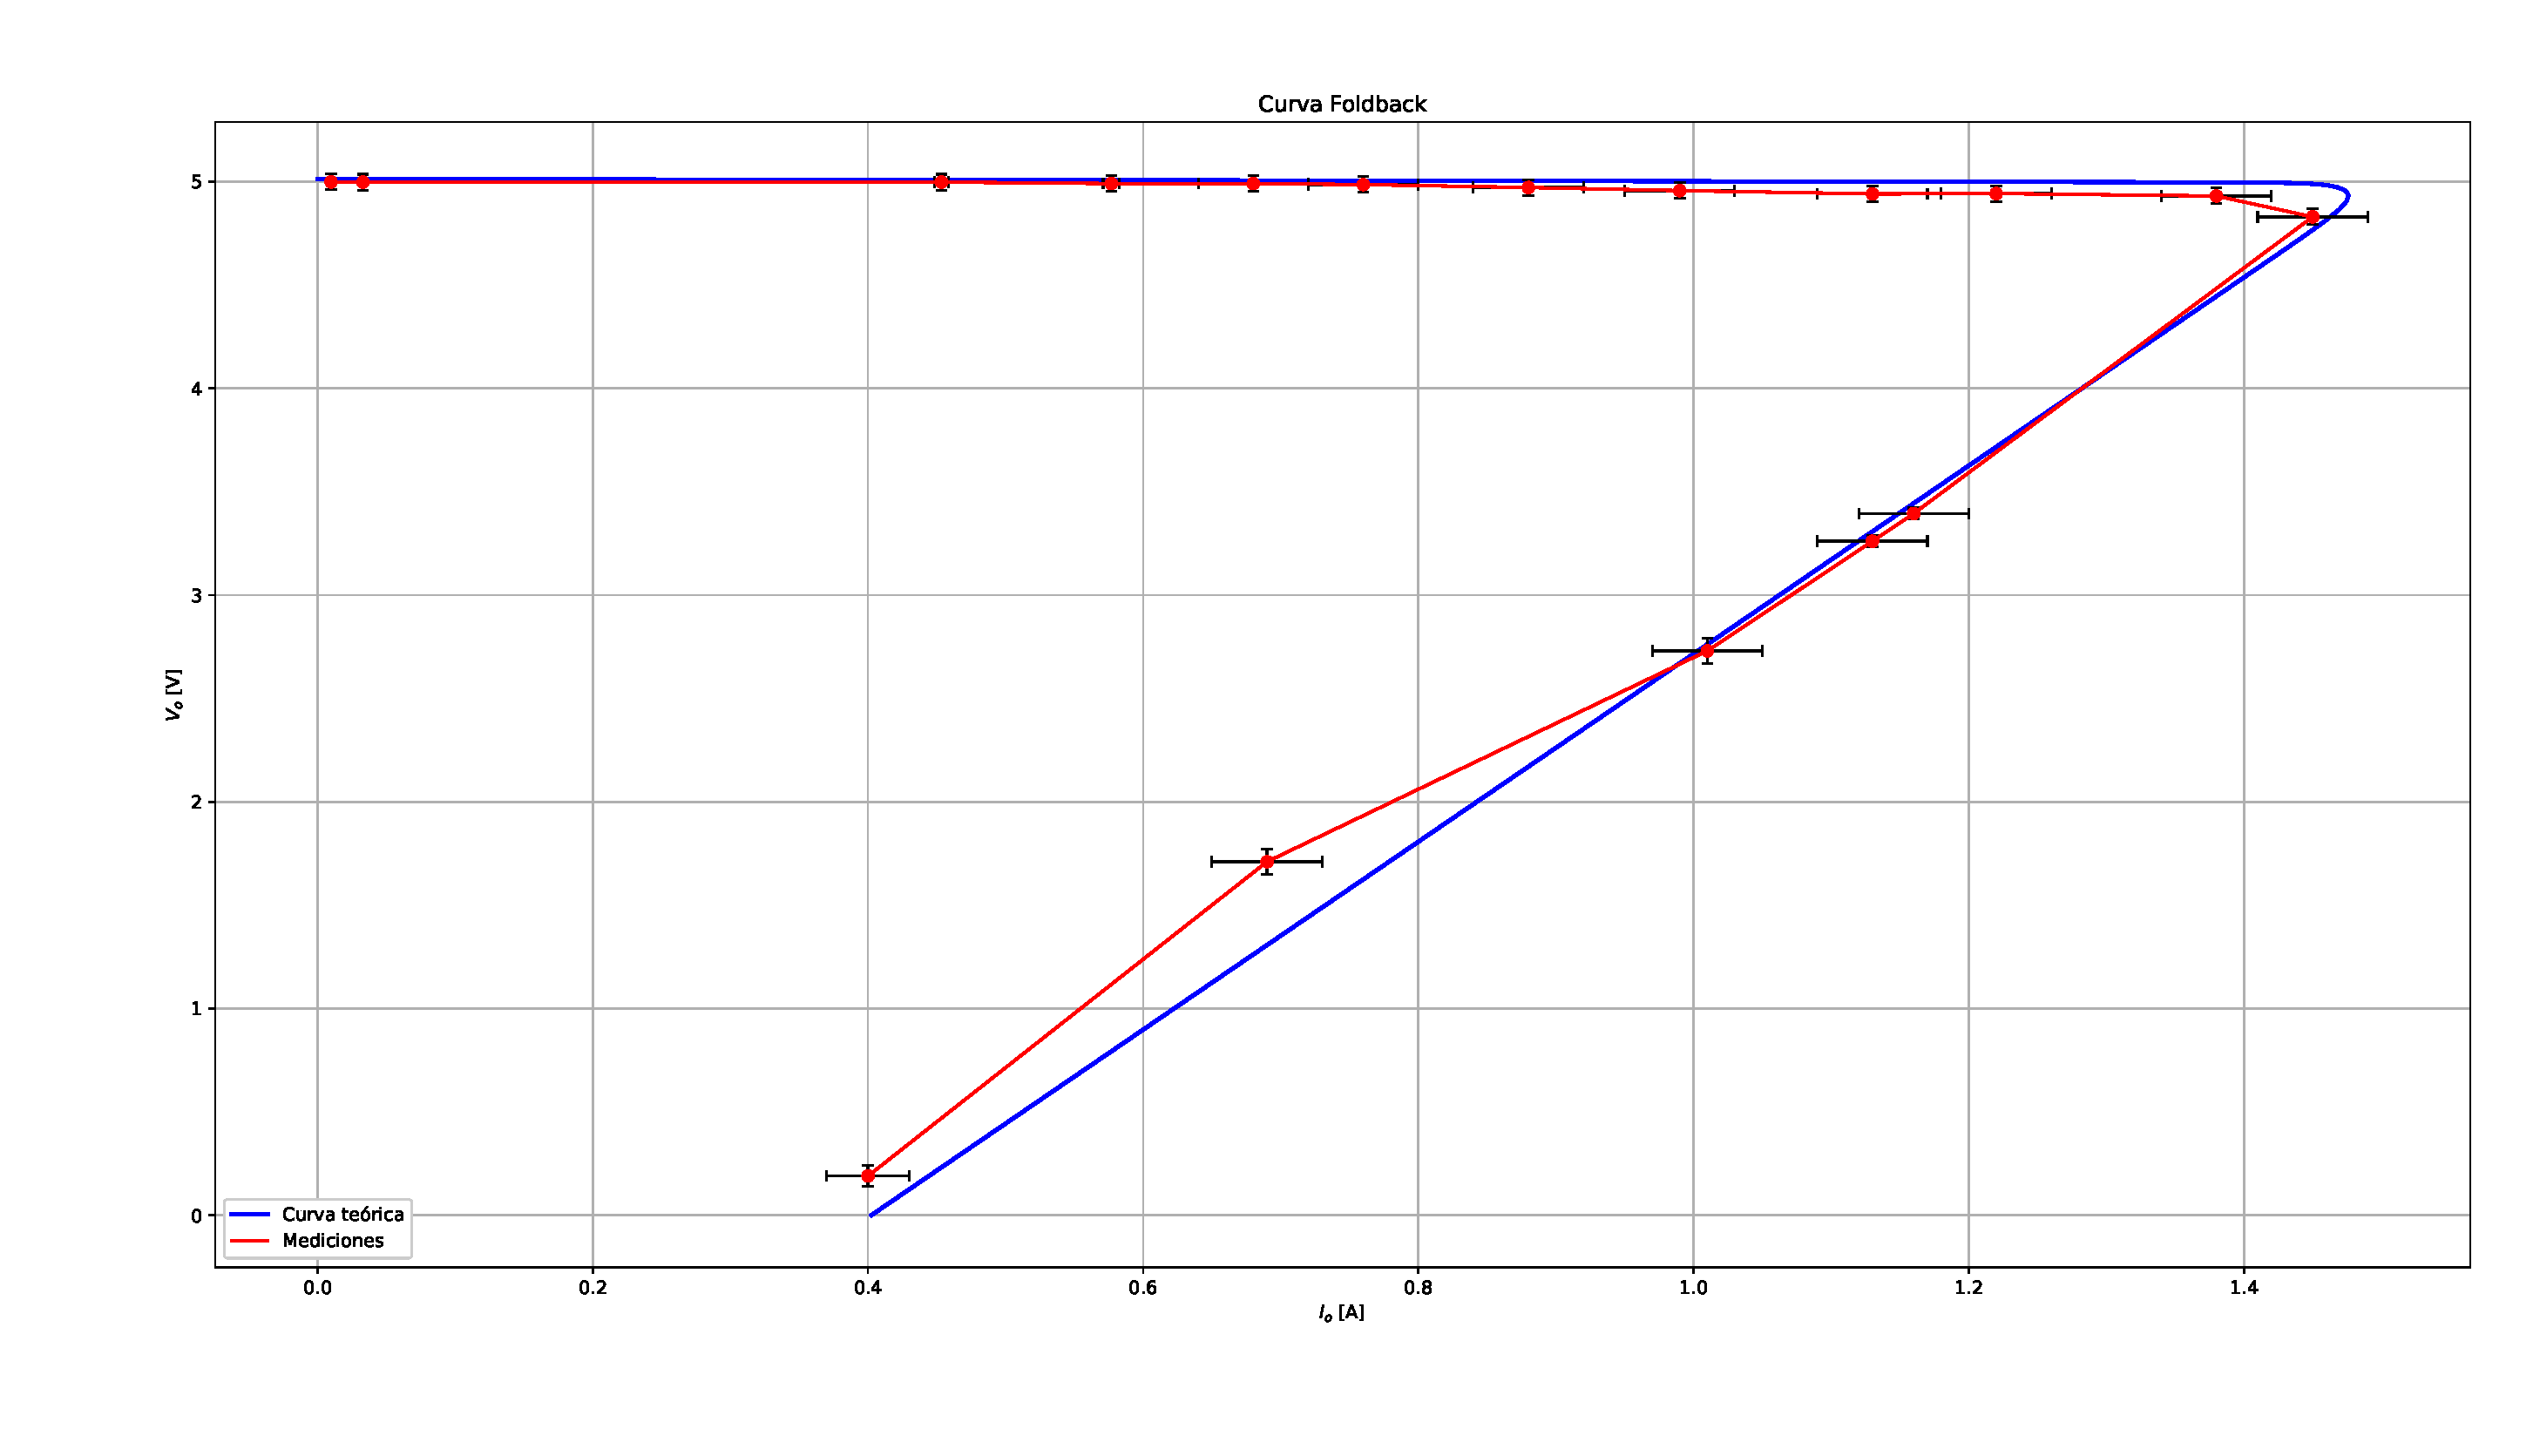
\includegraphics[width=\linewidth]{res/grafico_foldback.eps} 
    \caption{Foldback medido superpuesto al simulado} 
    \label{fig:foldback} 
\end{figure}
%%%%%%%%%%%%%%%%%%%%%%%%%%%%%%%%%%%%%%%%%%%%%%%%%%%%%%%%%%%%%%%%%%%%
\section{Eficiencia}
\begin{figure}[H] 
    \centering 
    \includegraphics[width=\linewidth]{res/grafico_eficiencia_corriente.eps} 
    \caption{Eficiencia contra corriente} 
    \label{fig:eficiencia_corriente} 
\end{figure}

\quad Primero se midió la eficiencia contra la corriente de salida, para esto se mantuvo la tensión de entrada en \SI{9.5}{V} y se hizo variar la carga entre los valores del rango de funcionamiento, midiendo las tensiones y corrientes tanto de entrada como de salida del circuito. 

\quad Como se puede ver en la curva de la \autoref{fig:eficiencia_corriente}, los valores rondan el 52\% de eficiencia, lo cual se corresponde con lo esperado. A bajas corrientes, la eficiencia cae porque la corriente de salida es del mismo orden que las corrientes internas de polarización, de modo que gran parte de la potencia de entrada no llega a la carga. Esto produce valores de eficiencia menores en el inicio de la curva.


\begin{figure}[H] 
    \centering 
    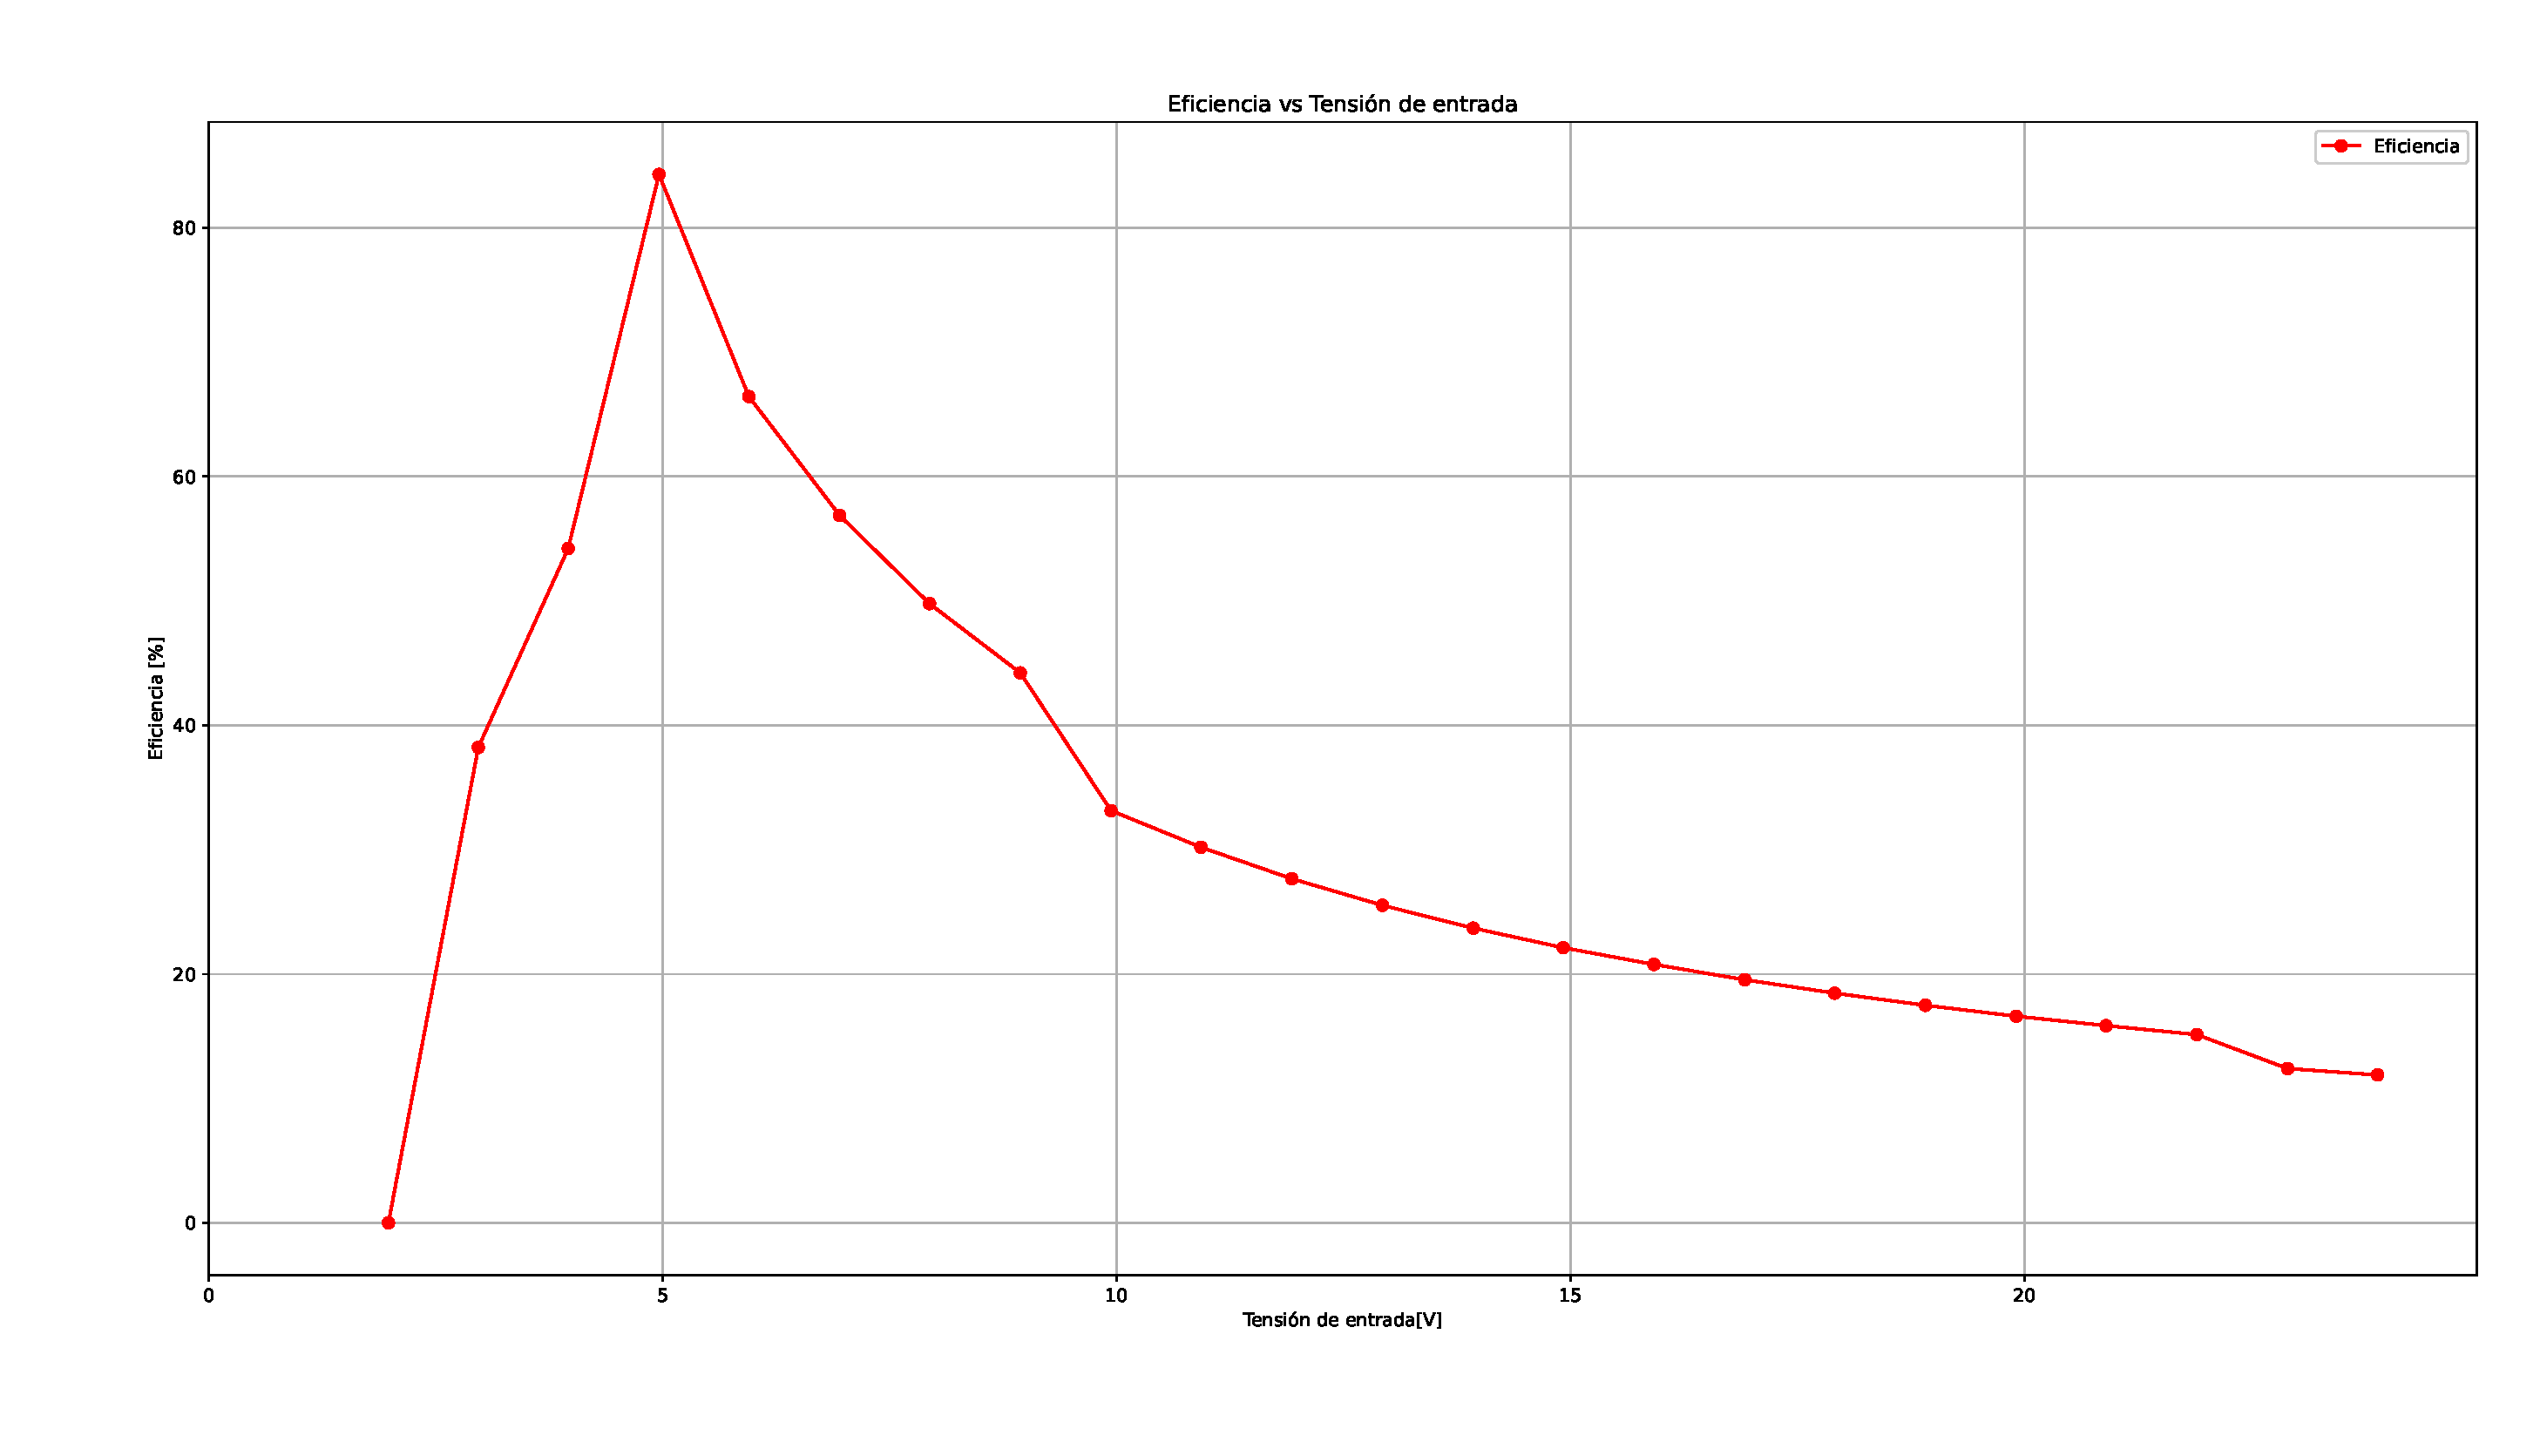
\includegraphics[width=\linewidth]{res/grafico_eficiencia_tension.eps} 
    \caption{Eficiencia contra tensión} 
    \label{fig:eficiencia_tension} 
\end{figure}

\quad Luego se midió la eficiencia contra la tensión de entrada, para esto se mantuvo la carga constante en \SI{100}{\ohm} y nuevamente se midieron las tensiones y corrientes de entrada como de salida, variando la tensión de entrada entre \SI{0}{V} y \SI{24}{V}.

\quad Como se puede ver en la \autoref{fig:eficiencia_tension}, la eficiencia presenta un pico en \SI{5}{V} de entrada, aunque en este caso no es utilizable el circuito, ya que la tensión de salida no se encuentra dentro de las especificaciones. Luego, el decrecimiento a medida que aumenta la tensión de entrada es esperable, ya que aumenta la potencia de entrada mientras que la potencia de salida se mantiene constante. 


%%%%%%%%%%%%%%%%%%%%%%%%%%%%%%%%%%%%%%%%%%%%%%%%%%%%%%%%%%%%%%%%%%%%
\section{Tiempo de respuesta}
\quad Al momento de medir el tiempo de encendido y apagado del circuito se utilizó una resistencia en paralelo con un capacitor de 10$\ohm$ y 1$\micro$F respectivamente. Para medirlo se debió conectar y desconectar la fuente de alimentación. Con un osciloscopio se utilizaron ambos canales, uno para observar el tiempo de respuesta de la desconexión de la fuente y otro para observar el tiempo de respuesta del circuito. Se consiguieron los siguientes gráficos. 
\begin{figure}[H] 
    \centering 
    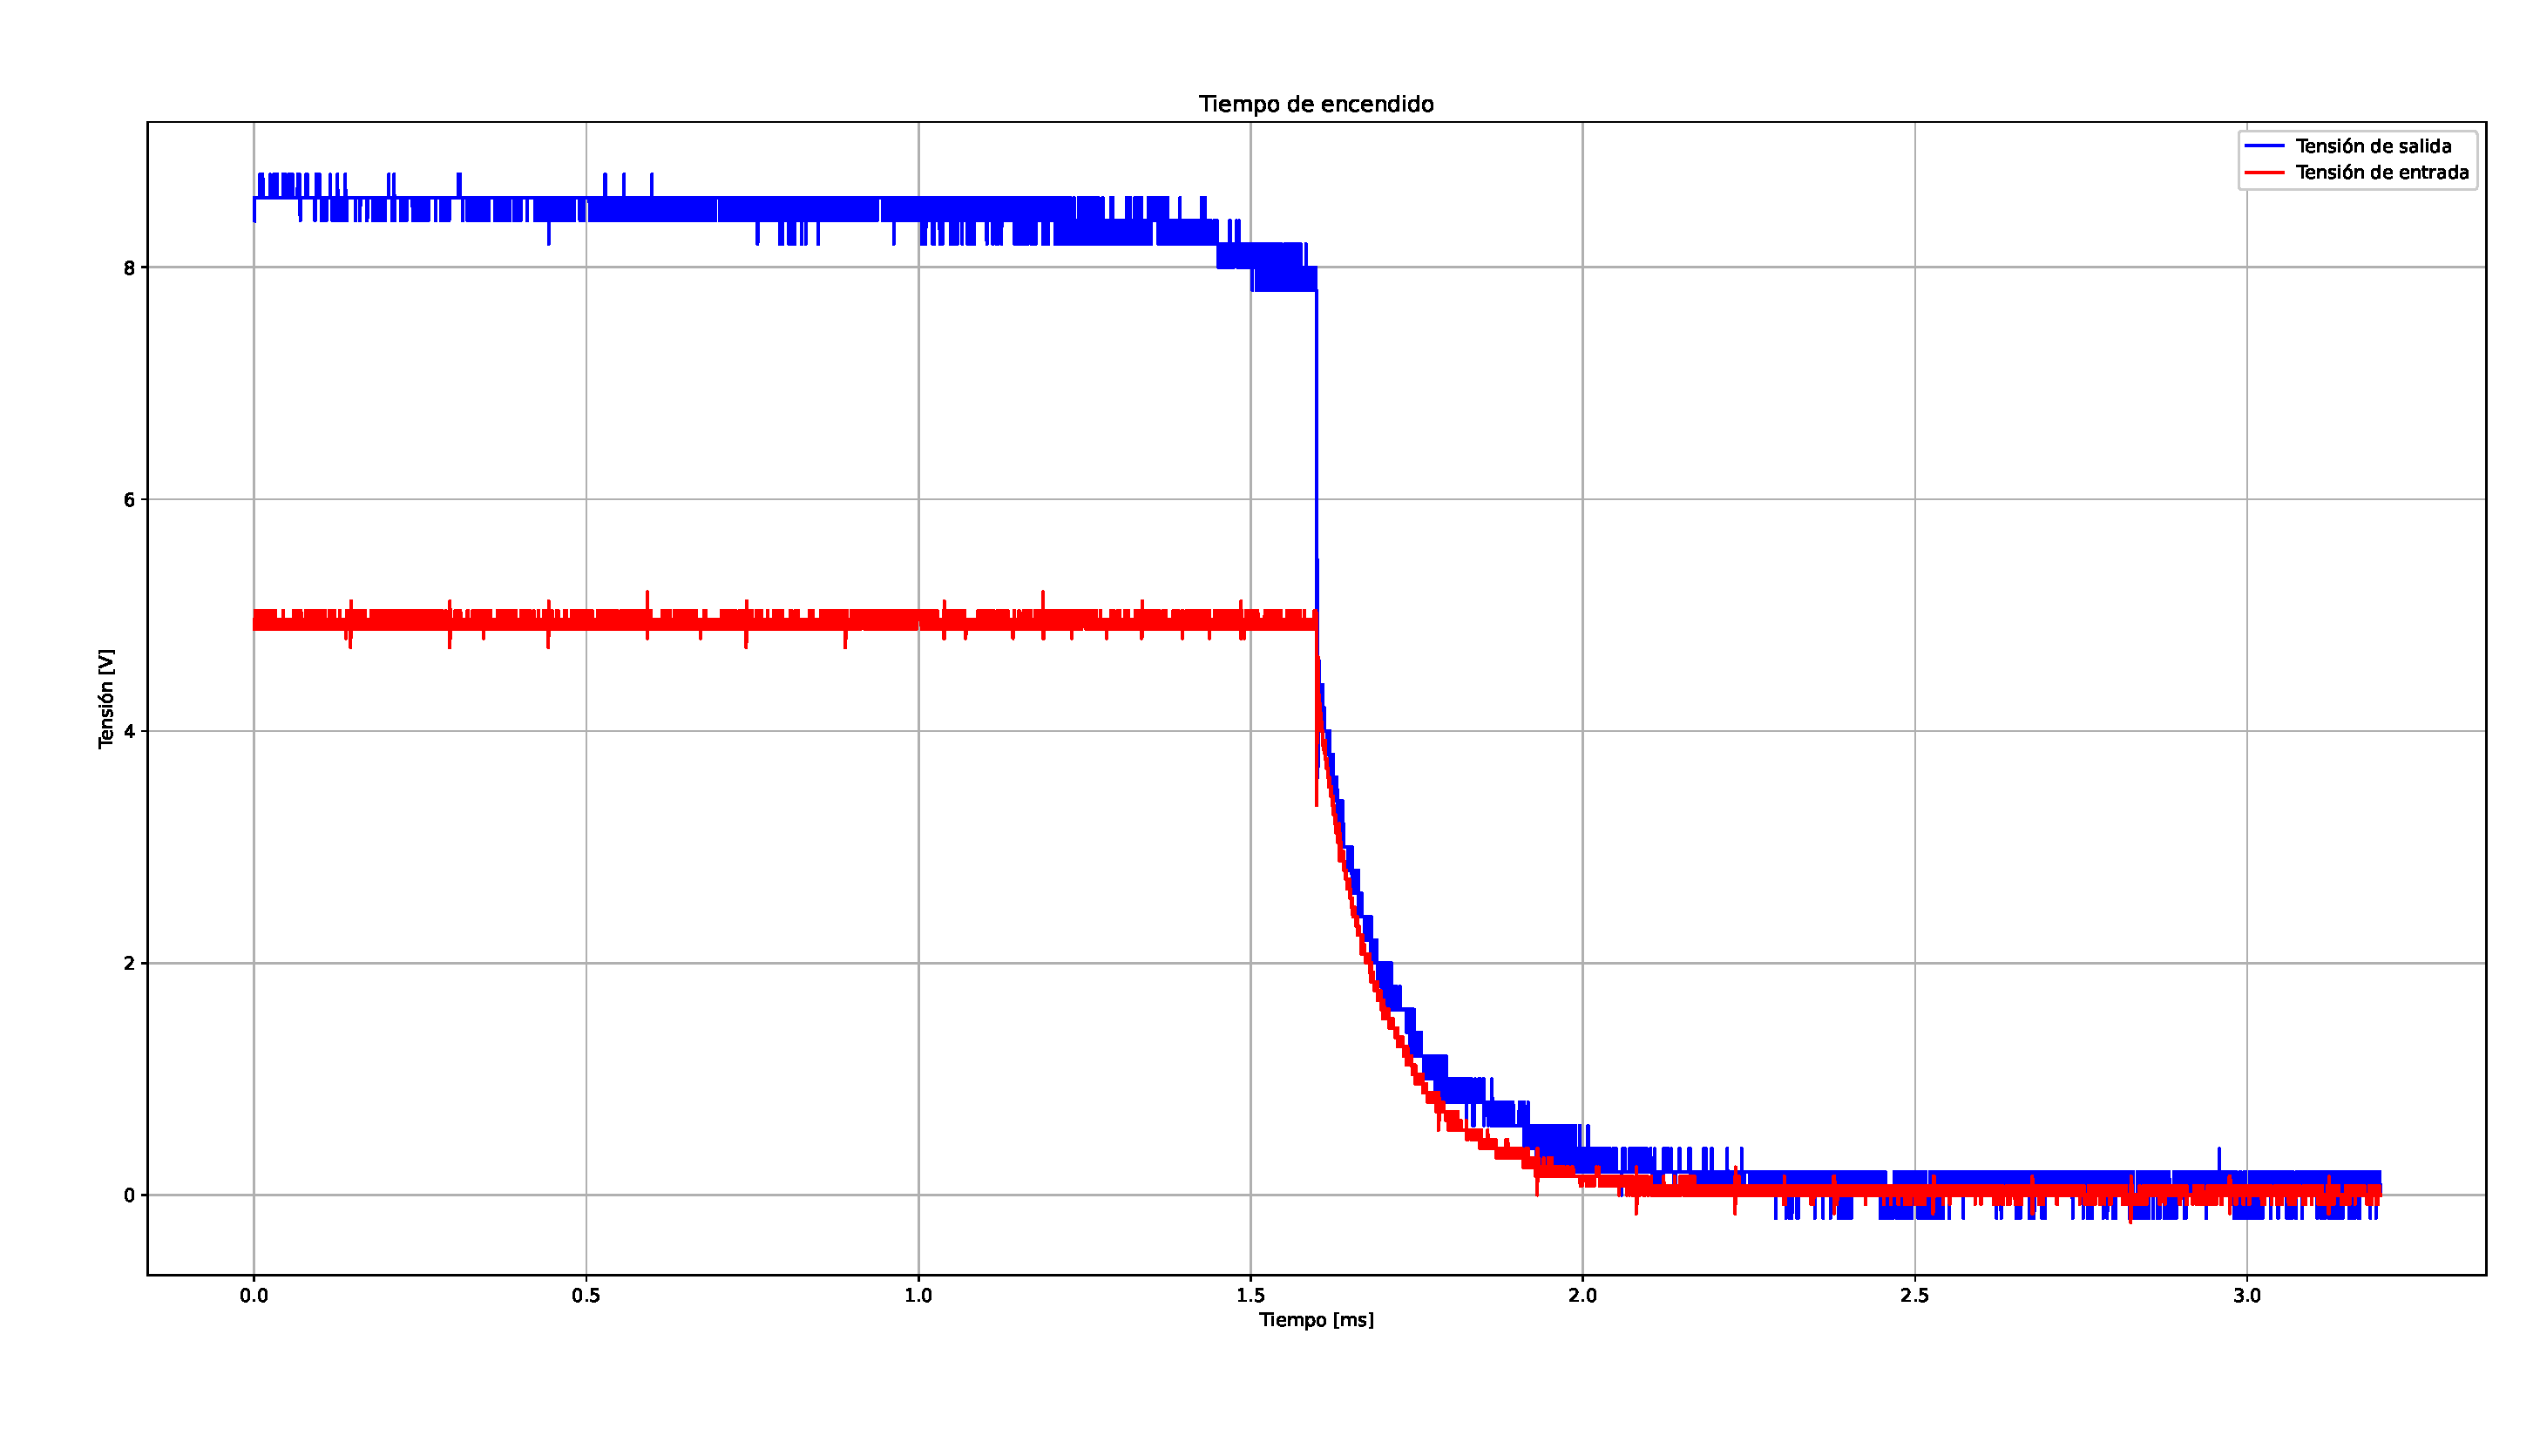
\includegraphics[width=\linewidth]{res/grafico_tiempo_apagado.eps} 
    \caption{Tiempo de respuesta apagado} 
    \label{fig:tiempo_apagado} 
\end{figure}

\begin{figure}[H] 
    \centering 
    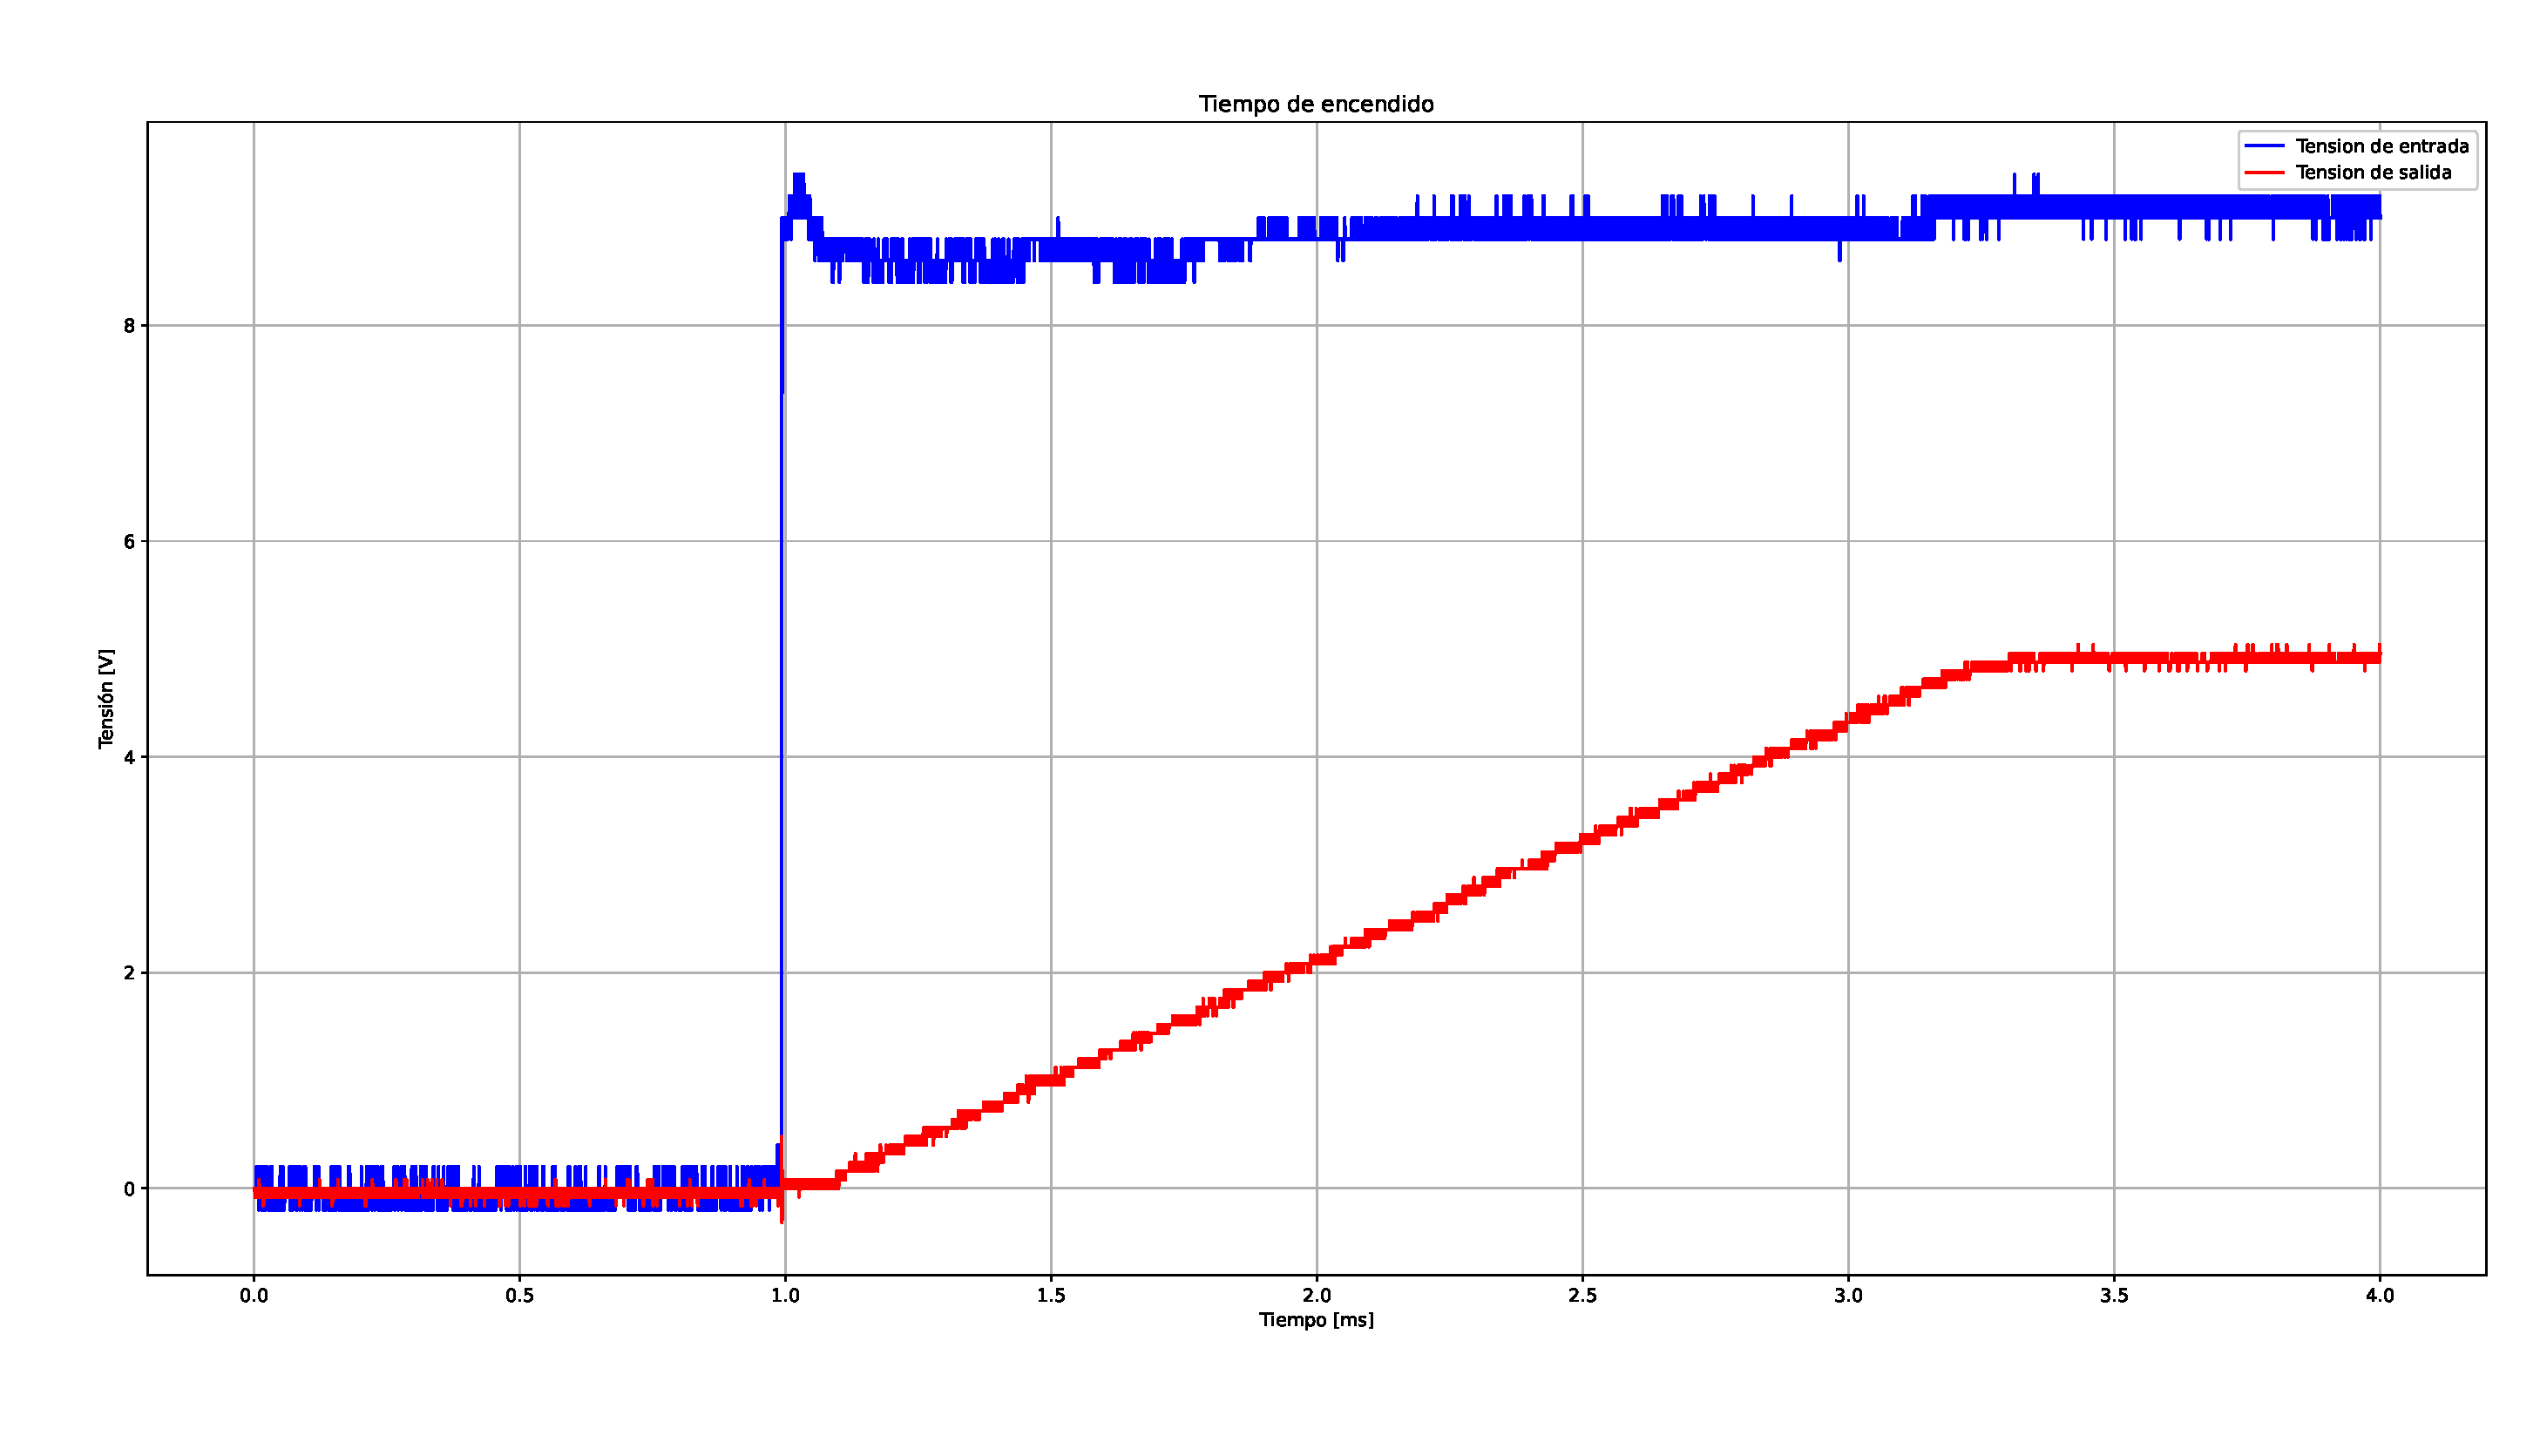
\includegraphics[width=\linewidth]{res/grafico_tiempo_encendido.eps} 
    \caption{Tiempo de respuesta encendido} 
    \label{fig:tiempo_encendido} 
\end{figure}

En la \autoref{fig:tiempo_apagado} se observa un tiempo de apagado de \SI{0.4}{ms}. En la \autoref{fig:tiempo_encendido} se observa un tiempo de encendido de \SI{2.5}{ms}. 

\begin{figure}[H] 
    \centering \includegraphics[width=\linewidth]{res/grafico_carga_dinamica.pdf} 
    \caption{Regulación de carga dinámica} \label{fig:reg_de_carga} 
\end{figure}

\quad En la \autoref{fig:reg_de_carga} se puede ver la respuesta ante una carga dinámica, en este caso pasando de una corriente de salida de \SI{128}{\milli \ampere} a una corriente de salida de \SI{406}{\milli \ampere}. Se puede ver que la tensión cae aproximadamente \SI{200}{\milli \volt}, pero se restablece luego de aproximadamente \SI{14}{\milli \second}.

%%%%%%%%%%%%%%%%%%%%%%%%%%%%%%%%%%%%%%%%%%%%%%%%%%%%%%%%%%%%%%%%%%%%
\section{Resultados}

A continuación se muestran los principales resultados obtenidos:

\begin{table}[h!]
    \centering
    \begin{tabular}{|c|c|c|}
    \hline
    Característica & Simulado & Medido      \\ \hline
    Tiempo de encendido   & $-$      & $2.5ms$      \\ \hline
    Tiempo de apagado     & $-$      & $0.4ms$       \\ \hline
    Regulación de linea   & $2.86$   & $1.75$         \\ \hline
    Regulación de carga    & $2.72m \ohm$ & $23.5m \ohm$  \\ \hline
    \end{tabular}
    \caption{Resultados}
    \label{tab:resultados}
\end{table}


\section{Conclusiones}


\quad En este trabajo se pudo armar el circuito diseñado en las entregas anteriores, verificando su funcionamiento dentro de las especificaciones y simulaciones. Las mediciones resultaron coherentes con lo diseñado, y en algunos casos hasta mejores que lo simulado. 
%%%%%%%%%%%%%%%%%%%%%%%%%%%%%%%%%%%%%%%%%%%%%%%%%%%%%%%%%%%%%%%%%%%%
\section{Anexo}
\subsection{Propagación de errores}

\quad Al momento de analizar los errores en la medición se debió tener en cuenta la dispersión de los multímetros y resistencias utilizados. Los multímetros con los que se realizaron las mediciones son: "UT890C", "UT139". Observando las especificaciones del fabricante se aprecia lo siguiente:
\begin{table}[h!]
\centering
\begin{tabular}{|c|c|c|}
\hline
\textbf{Magnitud} & \textbf{Rango} & \textbf{Resolución / Precisión} \\ \hline

\multirow{2}{*}{UT890C DC Current} 
& 600 mA & (1.2\% + 5) \\ \cline{2-3}
& 20 A & (2.0\% + 5) \\ \hline

\multirow{2}{*}{UT890C DC Voltage} 
& 600 mV & (0.5\% + 4) \\ \cline{2-3}
& 6 V &  (0.5\% + 2) \\ \hline

\multirow{1}{*}{UT139 DC Current} 
& 10 A & (0.7\% + 2) \\ \hline

\multirow{1}{*}{UT139 DC Voltage} 
& 600 V & (0.5\% + 2) \\ \hline

\end{tabular}
\caption{Incertezas de los multímetros UT890C y UT139}
\label{tab:incertezas-multimetros}
\end{table}

\quad Con esta tabla y suponiendo un error del 5\% en todas las resistencias ya es posible realizar el cálculo de propagación de errores para los diferentes casos.


\subsubsection{Error foldback}
\quad El error en la medición de foldback se calculó propagando el error de ambos multímetros y las resistencias para los diferentes valores de corriente y tensión. Se utilizó el UT890C para medir la corriente y el UT139 para medir la tensión. Entonces, el error estará dado por:

\quad $\Delta$ T + $\Delta$ I + $\Delta$ R

\quad Al momento de medir el error, se tomó que "Alta corriente" tiene una resolución de 0.01A y "Baja corriente" tiene una resolución de 0.1mA. El UT139 es de resolución variable. Existen cuatro casos de errores:

\quad 1. Alta tensión, baja corriente: \[
V = \big[(0.5\% V_{out} + 2) + 5\%R_L\big ]V 
\hspace{0.5cm} 
\text{y} 
\hspace{0.5cm} 
I = \big[(1.2\%I_{out} + 5) + 5\%R_L\big]A
\]


\quad 2. Alta tensión, alta corriente:  \[
V = \big[(0.5\%V_{out} + 2D) + 5\%R_L\big]V
\hspace{0.5cm}
\text{y}
\hspace{0.5cm}
I = \big[(2.0\%I_{out} + 5D) + 5\%R_L\big]A
\]

\quad 3. Baja tensión, alta corriente:  \[
V = \big[(0.5\%V_{out} + 2D) + 5\%R_L\big]V
\hspace{0.5cm}
\text{y}
\hspace{0.5cm}
I = \big[(2.0\%I_{out} + 5D) + 5\%R_L\big]A
\]

\quad 4. Baja tensión, baja corriente:  \[
V = \big[(0.5\%V_{out} + 2D) + 5\%R_L\big]V 
\hspace{0.5cm} 
\text{y} 
\hspace{0.5cm} 
I = \big[(1.2\%I_{out} + 5D) + 5\%R_L\big]I
\]


\end{document}